\chapter*{Appendix C:\\Sample Information}

\label{Sample_info}
\begin{figure}[]
\centering
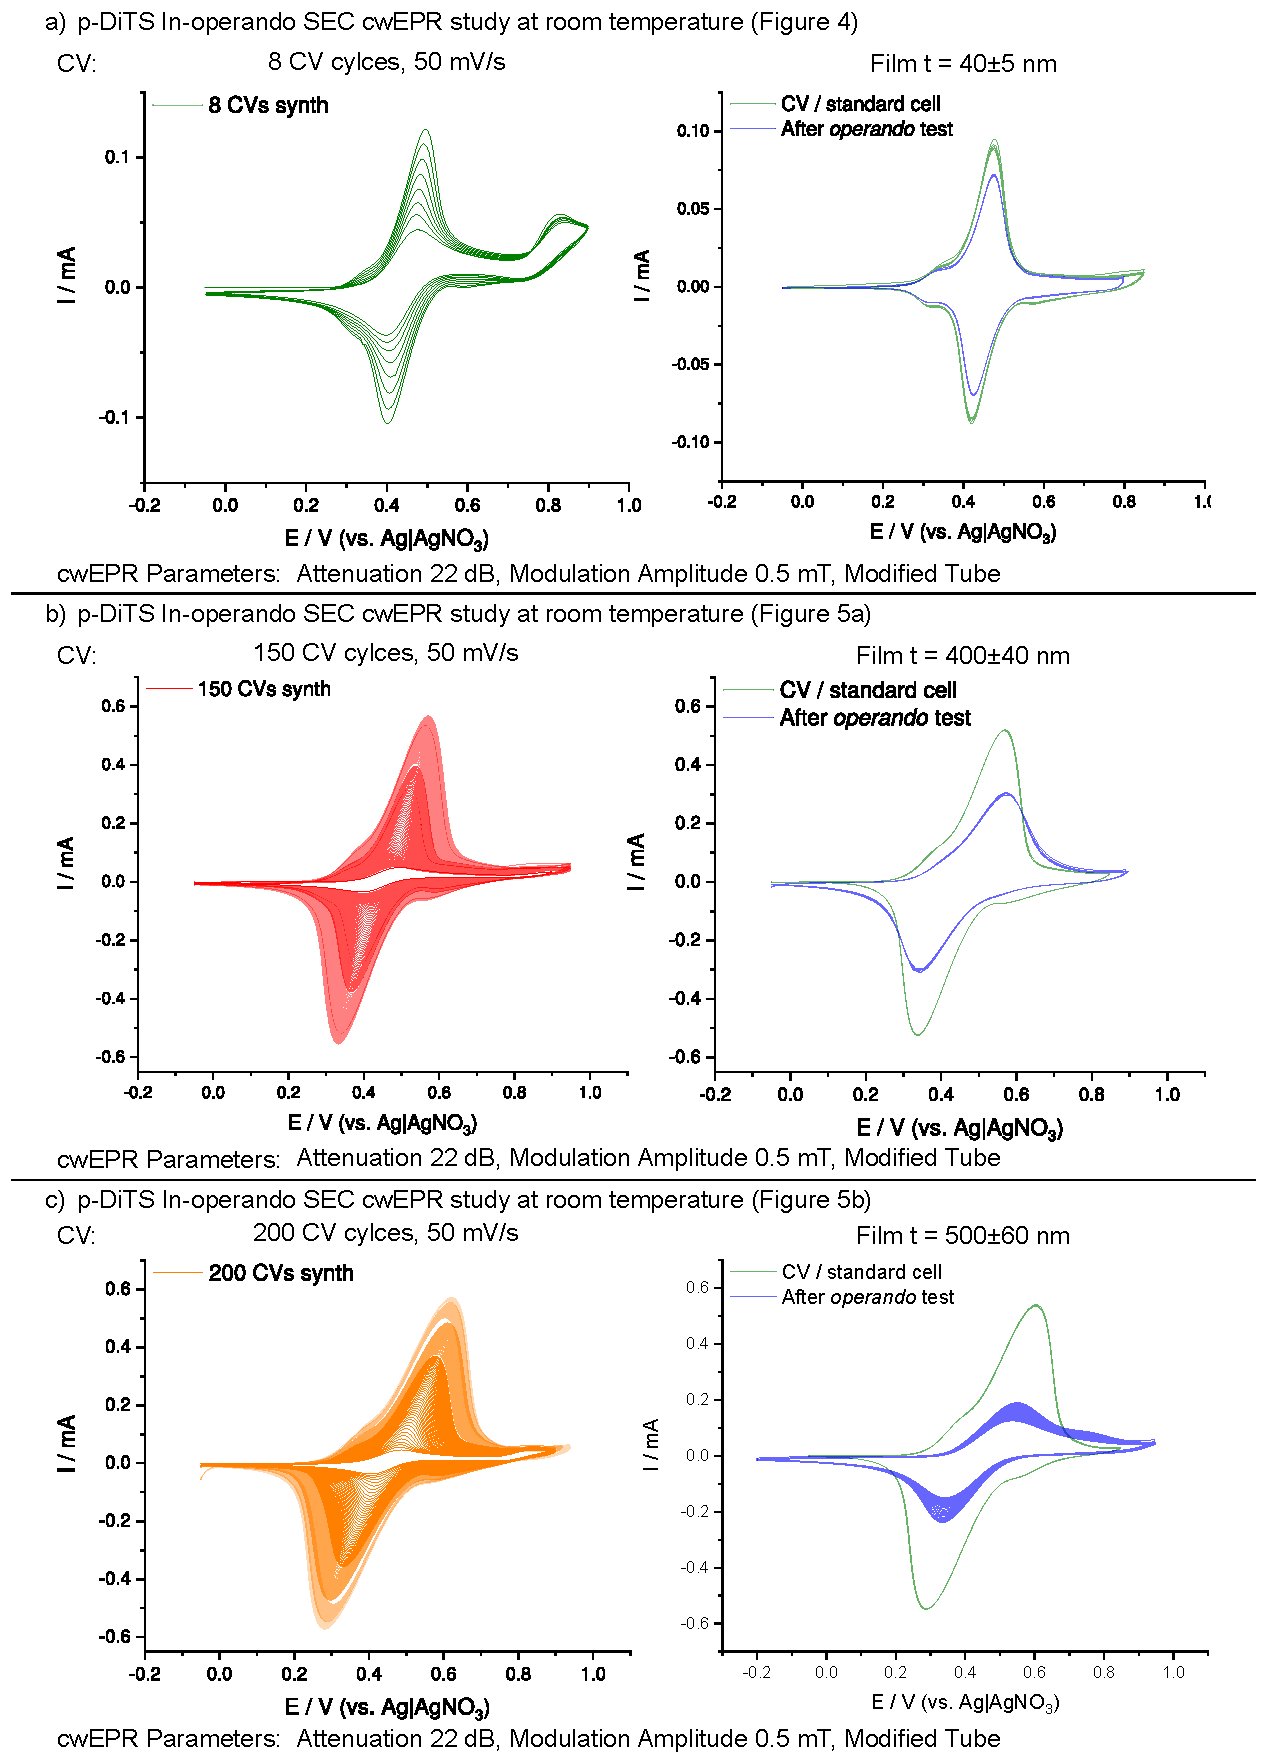
\includegraphics[width=0.93\textwidth]{./electrochemistry/figures/Figure_S3a}
%\caption{Sample information. Deposition curves, cycling curves, EPR parameters, figure references.}

\end{figure}
\newpage

\begin{figure}[]
\centering
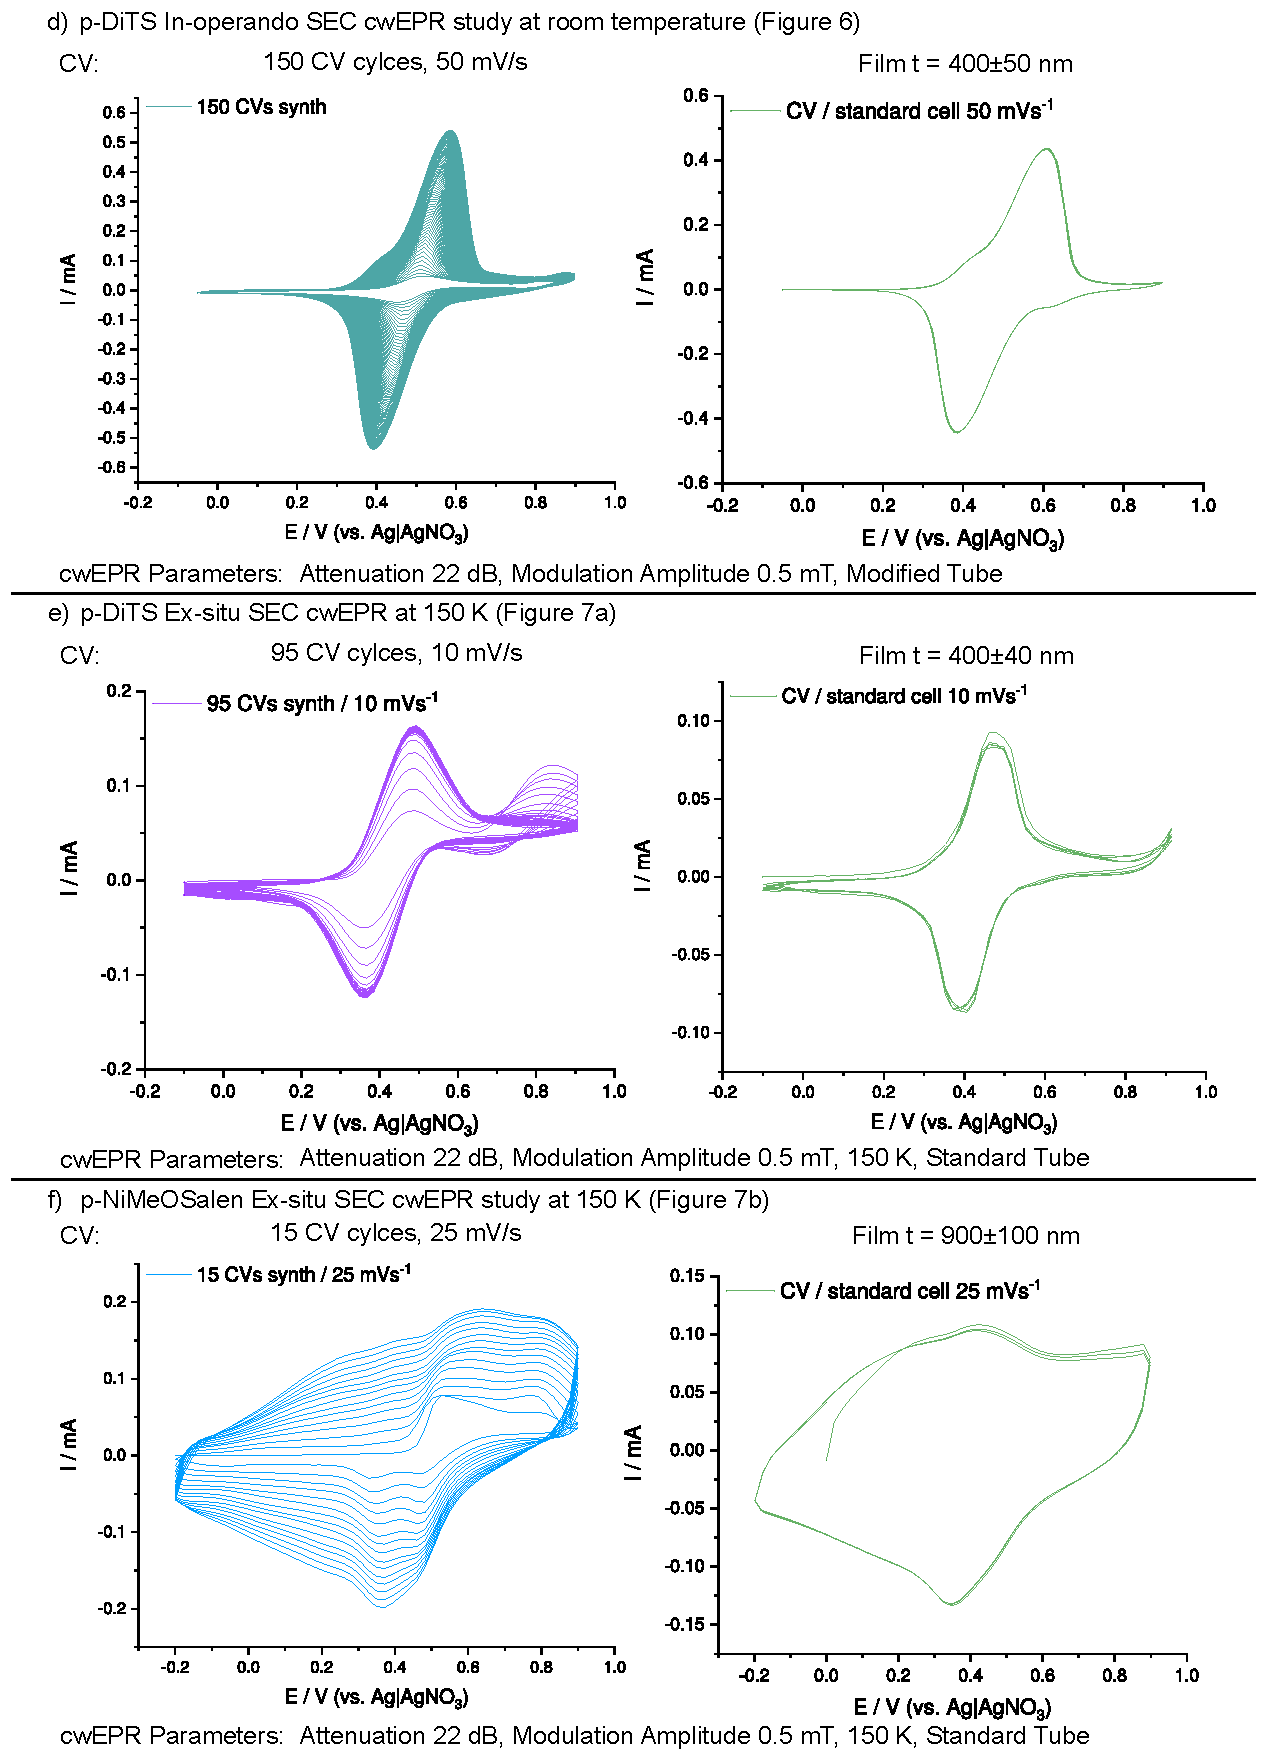
\includegraphics[width=0.93\textwidth]{./electrochemistry/figures/Figure_S3b}
\caption{Sample information. Deposition CV curves, Cleaning CV curves, EPR parameters, Figure references.}
\label{fig:S3}
\end{figure}

\newpage
\subsection*{Estimation of Cathode Film Thickness from Electrochemical Measurements}
\begin{figure}[H]
\center
	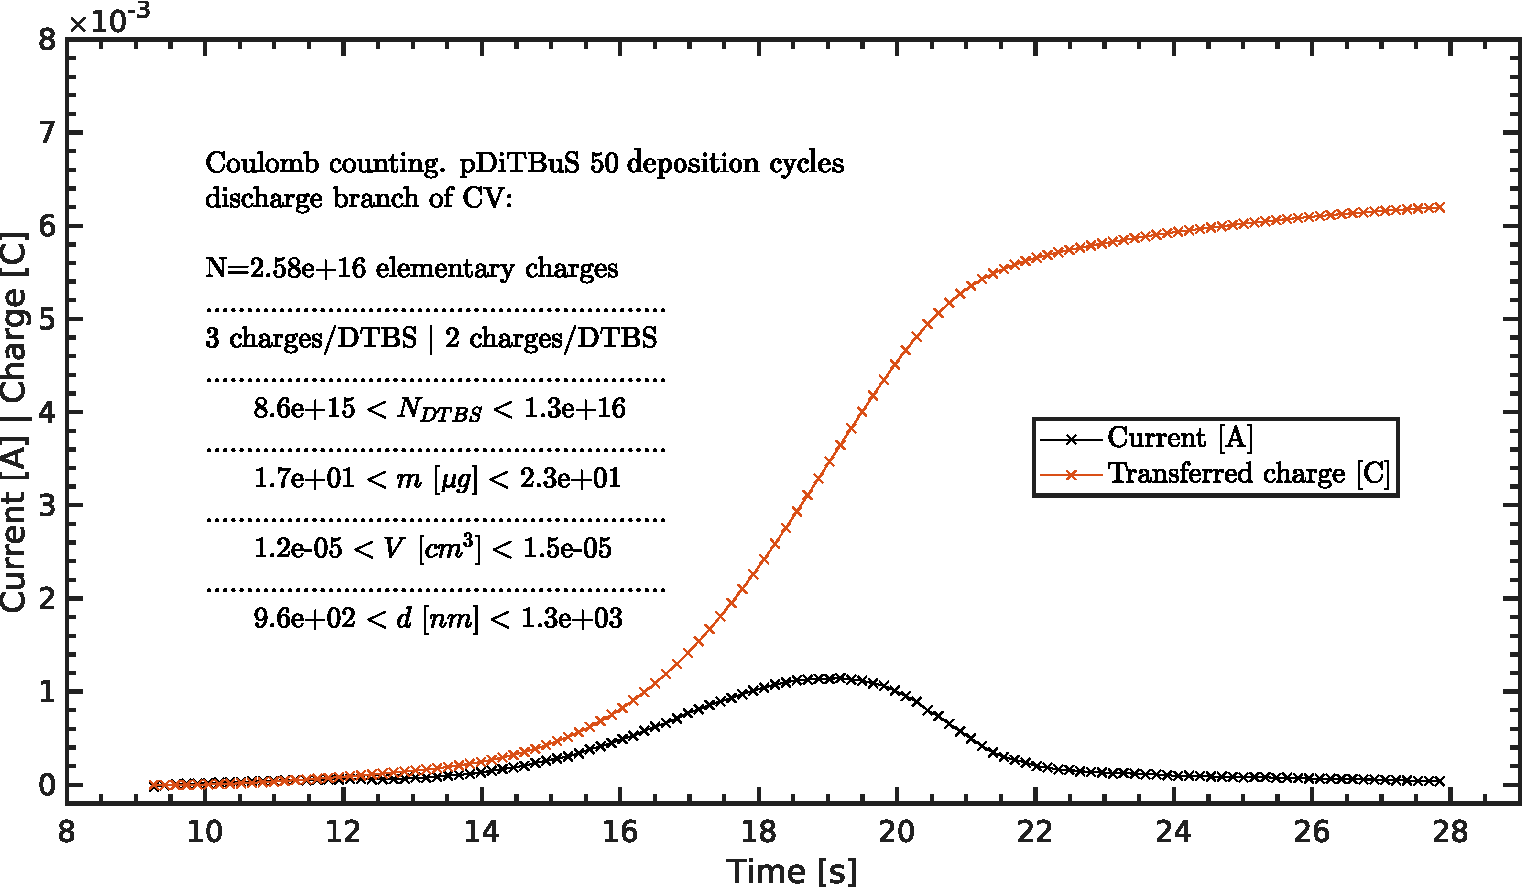
\includegraphics[width=1\textwidth]{./electrochemistry/figures/Figure_S28}
	\caption{\ik{Electrochemical determination of the number of DiTBuS units in the film, the mass, the volume and the thickness of the 50-CV pDiTBuS film. The transferred charge upon full oxidation was calculated with Coulomb counting. The calculated number of DiTBuS fragments in the film varies depending on whether one assumes only two-electron process during which only TEMPO moieties are being charged, or a three electron process, during which one positively charged polaron is additinally transferred to every DiTBuS fragment upon complete charging.}}
	\label{fig:Figure_S28}
\end{figure}

The volume of the film was calculated by integrating the discharge branch of the cyclic voltammogram to calculate the total charge of the film, then converting the charge to the number of DiTBuS monomer units assuming that all parts of the film are electrochemically active, and finally, converting the number of molecules to the volume using the density of pDiTBuS in the range between 1 and 2~g/cm$^3$. \ik{The corresponding curves and values are shown in Figure~\ref{fig:Figure_S28}}. The volume of the film was determined to be $\left(1.3\pm0.6\right)\times10^{-5}$cm$^{3}$.\\



